\chapter{Instrukcja użytkowania}
\section{Strona główna}
Strona główna~(zob.~rysunek~\ref{rys:main}) aplikacji została stworzona na bazie szablonu Bootstrap o nazwie One Page Wonder~\cite{opw}. Zawiera ona krótki opis aplikacji, a także korzyści płynących z wykorzystania jej dla planistów, nauczycieli oraz uczniów. Pasek menu znajdujący się zawsze na górze strony jest stałym elementem aplikacji pojawiającym się w każdym z widoków. Pozwala on na przejście do widoków logowania i rejestracji, a w przypadku gdy użytkownik jest już zalogowany na wylogowanie lub przejście do widoku szkoły. 
\begin{figure}[!ht]
\centering
\includegraphics[width=\textwidth]{figures/main}
\caption{Aplikacja internetowa -- Strona główna}\label{rys:main}
\end{figure}
\section{Widok szkoły}
Widok szkoły~(zob.~rysunek~\ref{rys:school}) pozwala na przejście do dodawania danych potrzebnych do wygenerowania planu, a przypadku gdy plan został już wygenerowany jest również miejscem, w którym jest on wyświetlany. Rozkład zajęć jest możliwy do wyświetlenia na trzy sposoby -- z podziałem na klasy, nauczycieli lub sale lekcyjne.

\begin{figure}[!ht]
\centering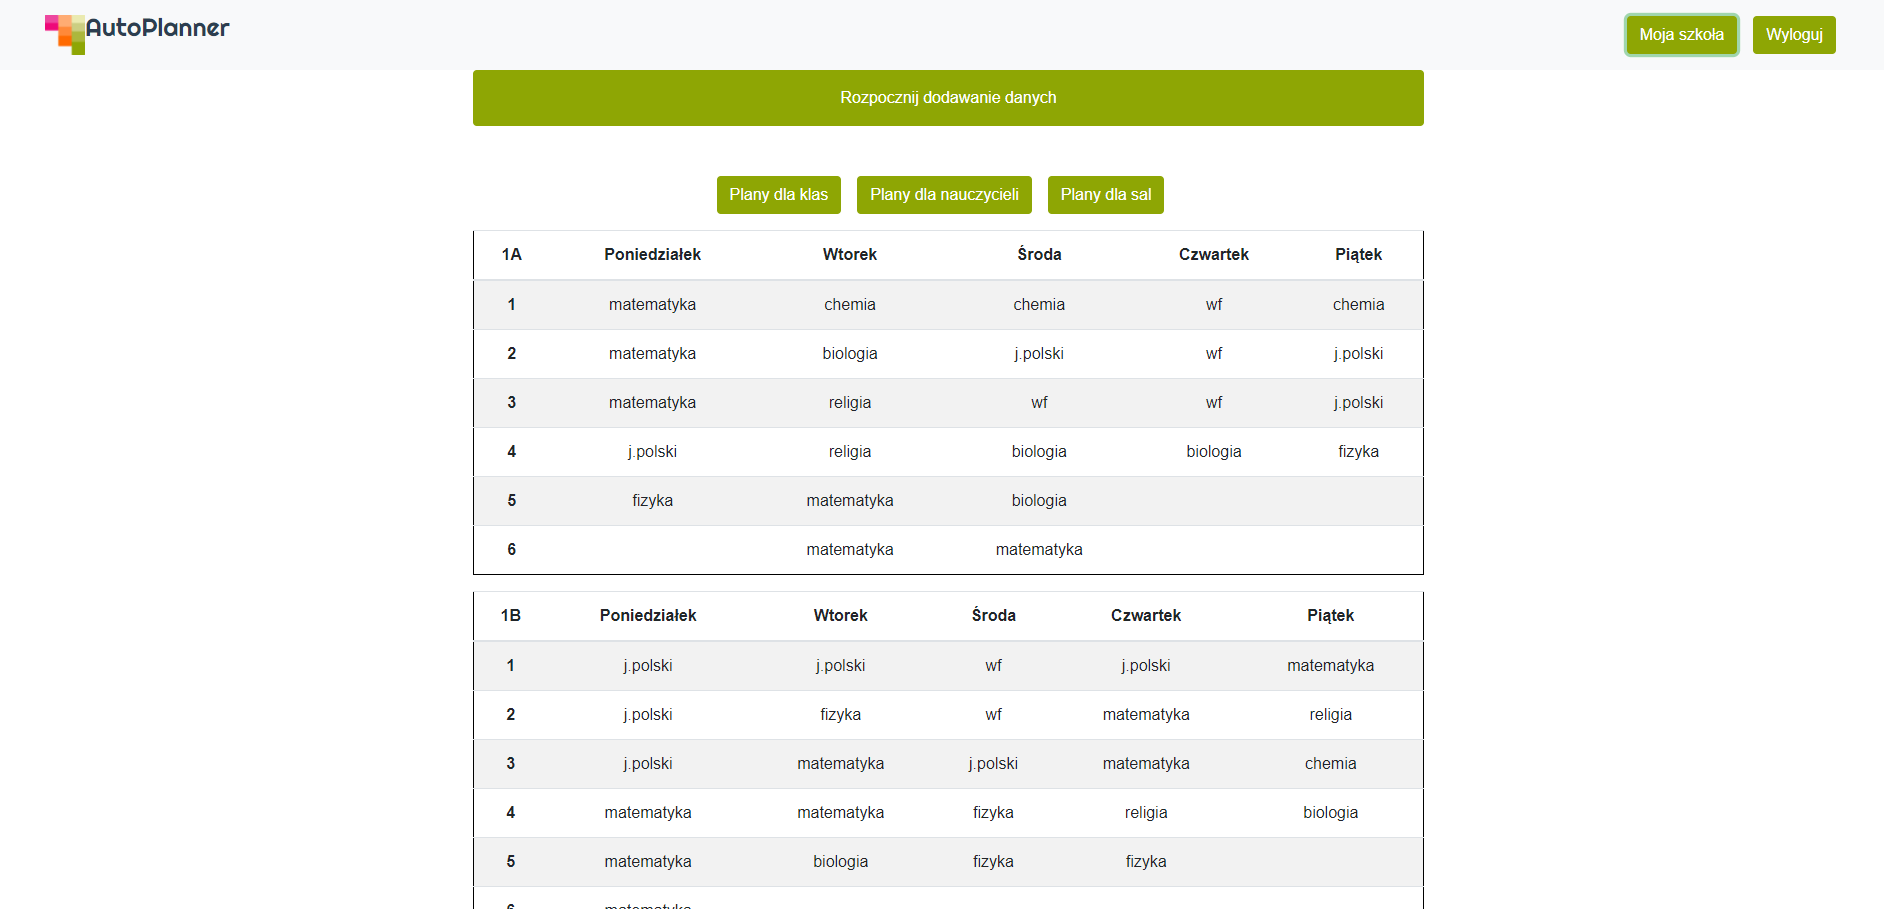
\includegraphics[width=\textwidth]{figures/school}
\caption{Aplikacja internetowa -- Widok szkoły}\label{rys:school}
\end{figure}
\section{Rejestracja}
Widok rejestracji~(zob.~rysunek~\ref{rys:register}) umożliwia utworzenie konta w serwisie. Od użytkownika wymaga się podania adresu e-mail, nazwy użytkownika oraz hasła. Adres e-mail musi być unikatowy. Wynika to z konieczności weryfikacji konta poprzez wiadomość wysłaną przy pomocy serwera SMTP. Rozwiązanie to ma na celu zapobieganie atakom na stronę poprzez masowe tworzenie nowych kont. 
\begin{figure}[!ht]
\centering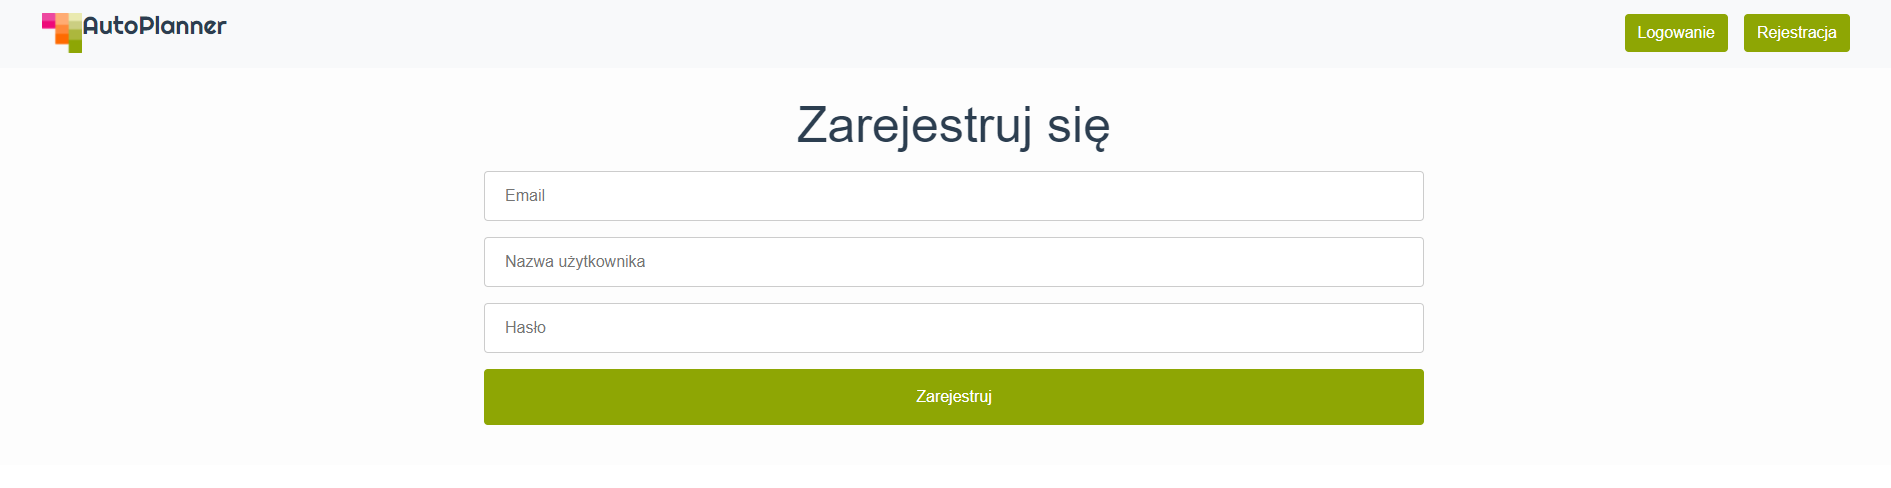
\includegraphics[width=\textwidth]{figures/register}
\caption{Aplikacja internetowa -- Widok rejestracji}\label{rys:register}
\end{figure}
\section{Logowanie}
Widok logowania~(zob.~rysunek~\ref{rys:login}) pozwala na dostęp do konta i zapisanych na nim danych z dowolnego urządzenia. Do uwierzytelnienia użytkownika wykorzystywany jest adres e-mail oraz hasło podane w procesie rejestracji. Powodzenie procesu logowania powoduje otrzymanie przez aplikację tokenu JWT, zapisywanego w pamięci przeglądarki. W przypadku utraty hasła użytkownik posiada możliwość odzyskania go po podaniu adresu e-mail powiązanego z istniejącym kontem.
\begin{figure}[!ht]
\centering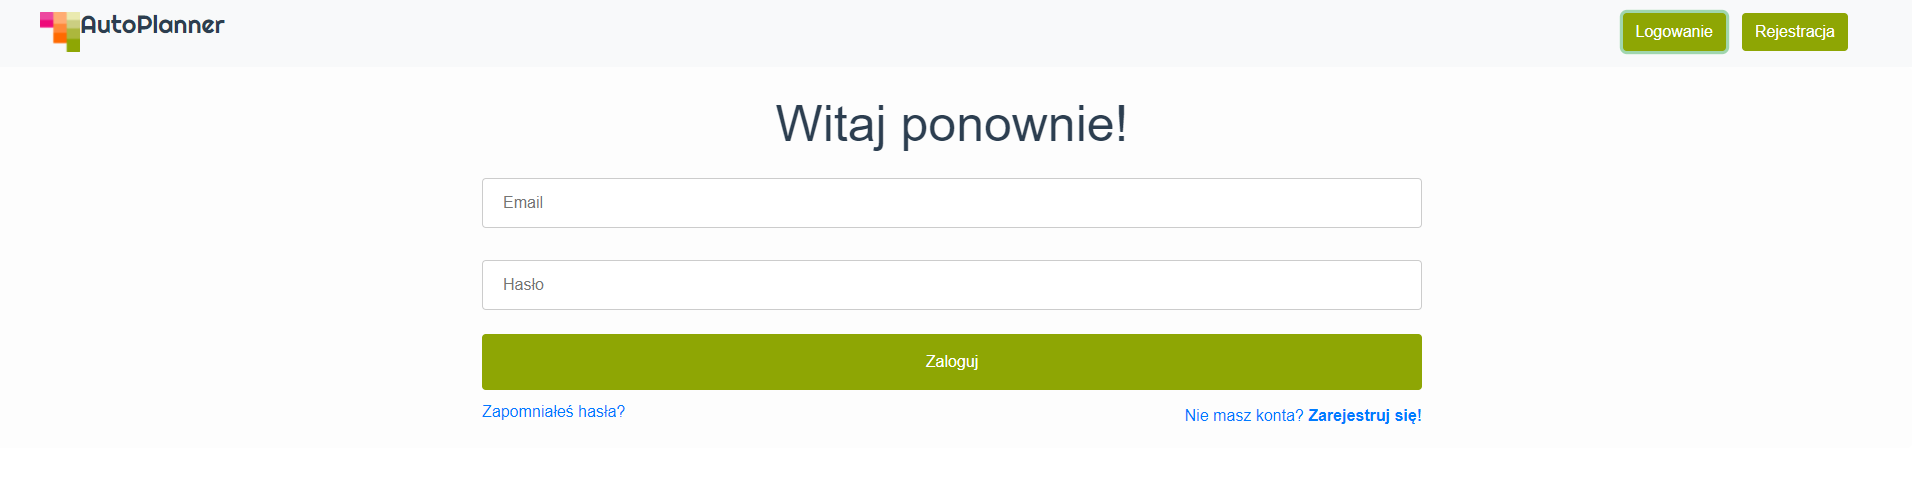
\includegraphics[width=\textwidth]{figures/login}
\caption{Aplikacja internetowa -- Widok logowania}\label{rys:login}
\end{figure}
\section{Ankieta}
Widok ankiety~(zob.~rysunek~\ref{rys:poll}) pozwala nauczycielowi na podanie preferencji godzinowych pracy. W przeciwieństwie do pozostałych widoków jest on dostępny jedynie poprzez bezpośredni link wysyłany w wiadomości e-mail. Takie rozwiązanie sprawia, że jedynym użytkownikiem, od którego wymagane jest posiadanie konta jest planista. Nauczyciele jako użytkownicy bez konta są identyfikowani dzięki unikalności adresu URL.
\begin{figure}[!ht]
\centering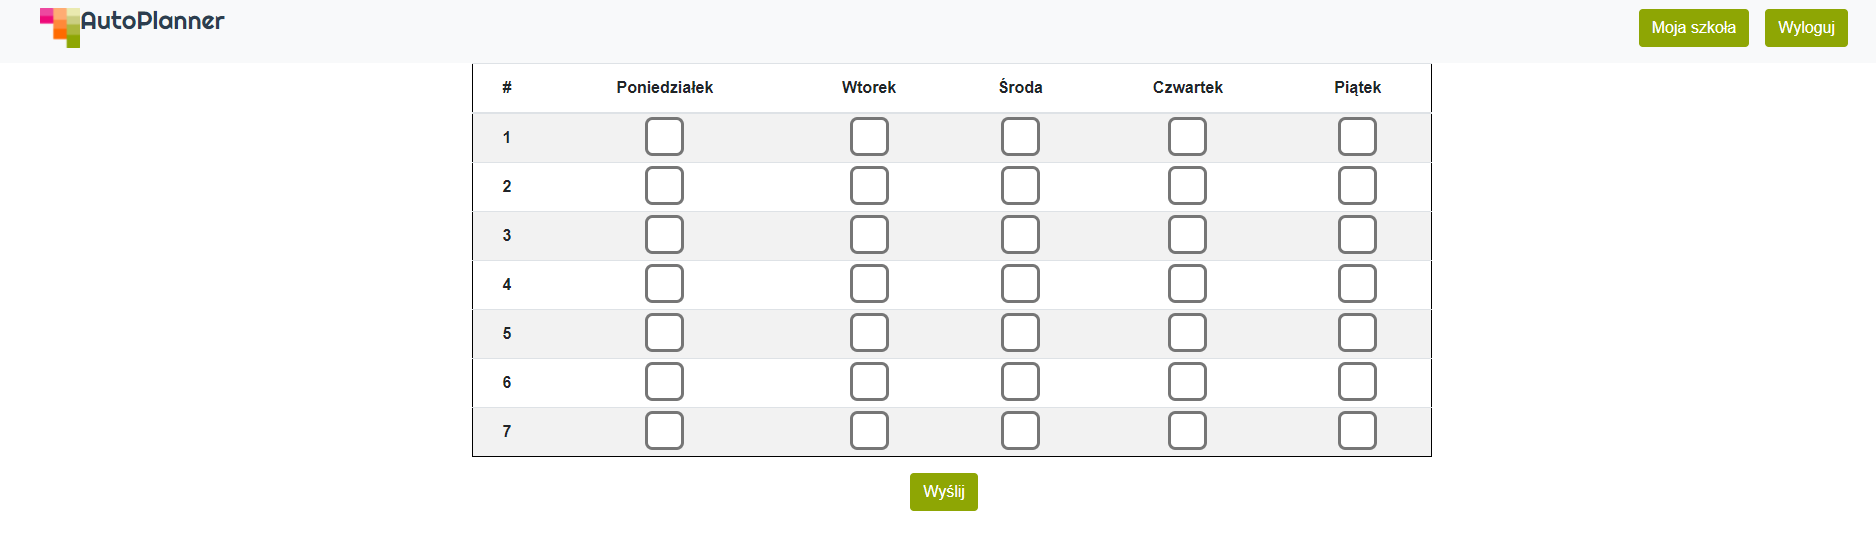
\includegraphics[width=\textwidth]{figures/poll}
\caption{Aplikacja internetowa -- Widok ankiet dla nauczycieli}\label{rys:poll}
\end{figure}
\section{Dodawanie przedmiotów}
Widok dodawania przedmiotów~(zob.~rysunek~\ref{rys:subject}) stanowi pierwszy krok w procesie podawania danych koniecznych do wygenerowania planu zajęć. W celu dodawania przedmiotu należy podać jedynie jego nazwę. Powiązania z nauczycielami, salami lekcyjnymi i klasami będą mogły być wprowadzone w kolejnych krokach. Podanie nazw przedmiotów na początku procesu dodawania danych pozwala na to, aby w późniejszych etapach mogły być one wybierane z listy rozwijanej. Zapobiega to konieczności wielokrotnego ręcznego wprowadzania tych samych informacji i ułatwia tworzenie powiązań w bazie danych. W lewej części ekranu znajduje się lista już wprowadzonych przedmiotów. Wybranie z nich jednego powoduje przejście do ekranu edycji. Analogiczne rozwiązanie zostało zastosowane we wszystkich kolejnych ekranach dodawania danych.
\begin{figure}[!ht]
\centering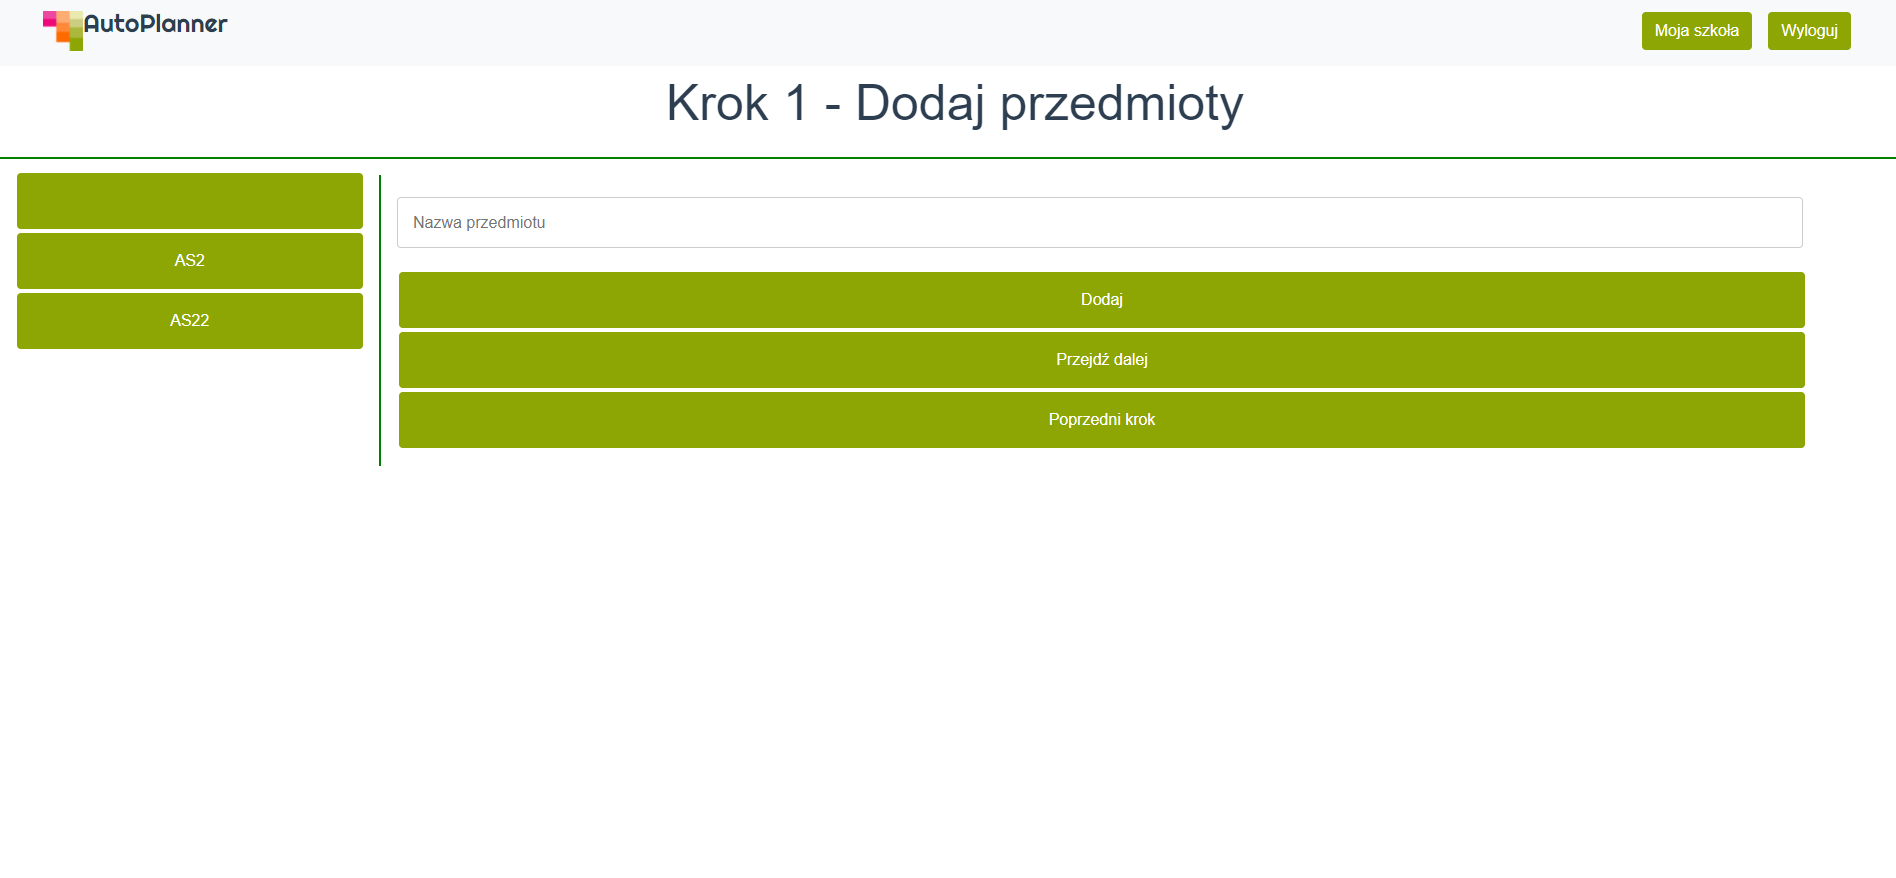
\includegraphics[width=\textwidth]{figures/subject}
\caption{Aplikacja internetowa -- Widok dodawania przedmiotów}\label{rys:subject}
\end{figure}
\section{Dodawanie nauczycieli}
W widoku dodawania nauczycieli~(zob.~rysunek~\ref{rys:teacher}) planista ma możliwość wprowadzenia danych personelu dydaktycznego oraz jego powiązań z przedmiotami. Każdy nauczyciel musi posiadać imię i nazwisko, unikalny w skali szkoły adres e-mail oraz przynajmniej jeden prowadzony przedmiot. Ekran umożliwia dodanie kolejnych prowadzonych przedmiotów w przypadku, gdy nauczyciel prowadzi więcej niż jeden. 
\begin{figure}[!ht]
\centering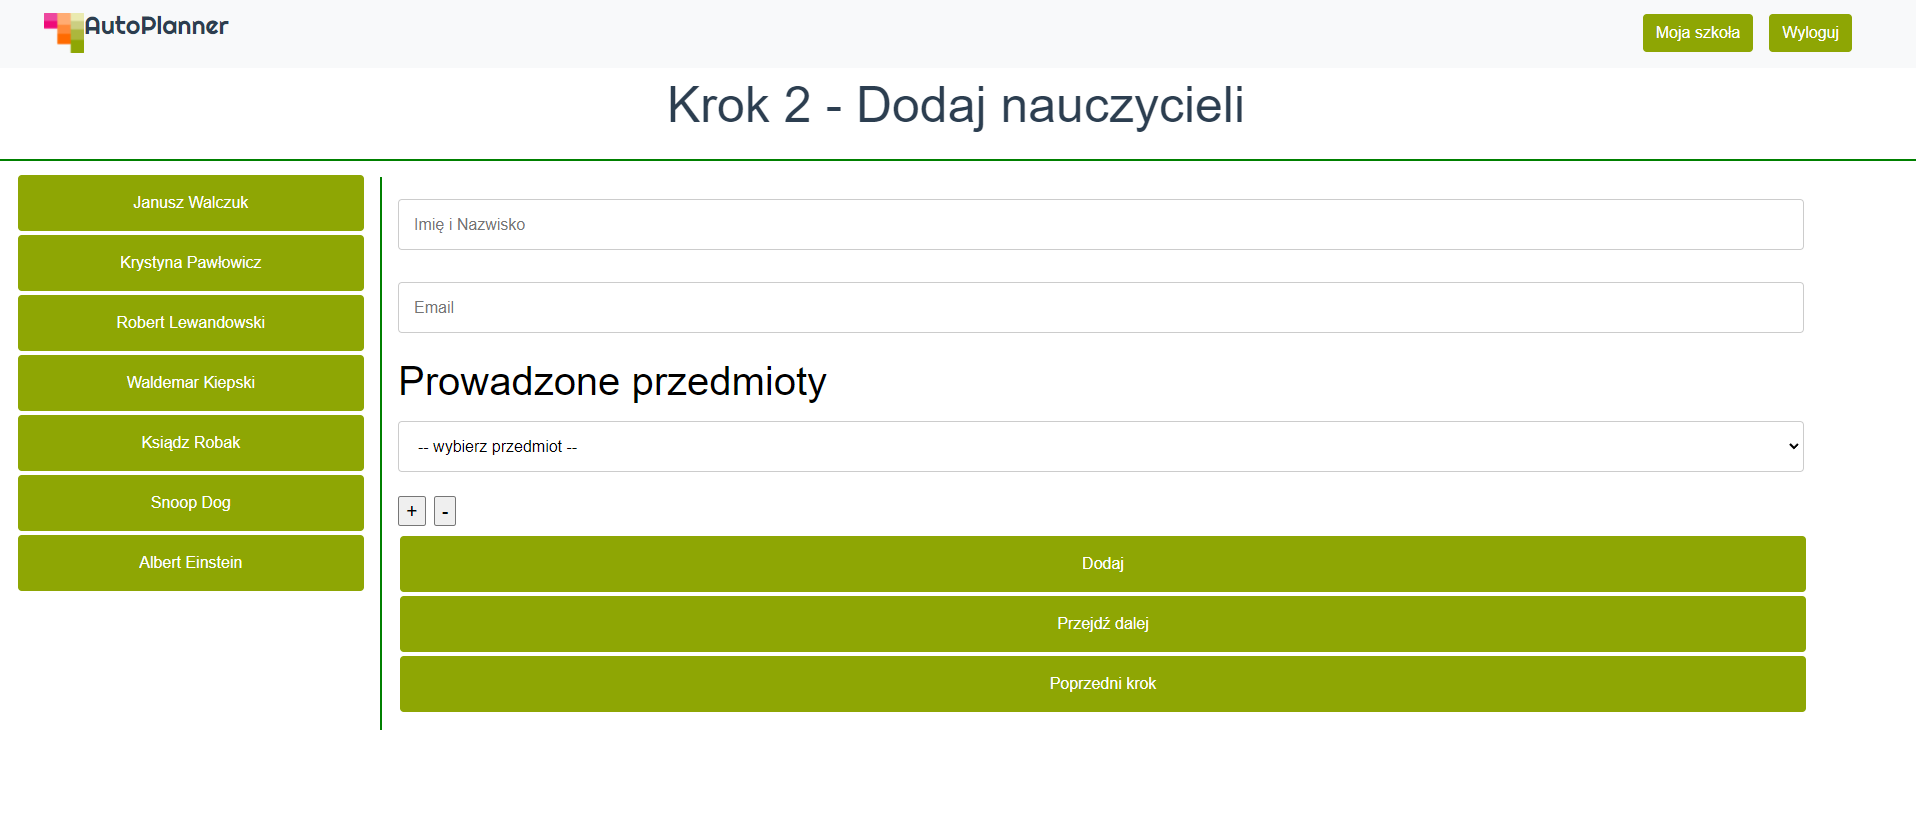
\includegraphics[width=\textwidth]{figures/teacher}
\caption{Aplikacja internetowa -- Widok dodawania nauczycieli}\label{rys:teacher}
\end{figure}
\section{Dodawanie sali lekcyjnych}
Dodanie informacji o salach lekcyjnych~(zob.~rysunek~\ref{rys:classroom}) stanowi trzeci krok dodawania danych. Sala lekcyjna musi posiadać nazwę, a opcjonalnie także listę przedmiotów, które mogą być w  niej prowadzone. W przypadku, gdy nie zostanie wybrany żaden preferowany przedmiot, sala zostaje uznana za salę zwykłą, co oznacza, że będzie mógł być w niej prowadzony dowolny przedmiot.
\begin{figure}[!ht]
\centering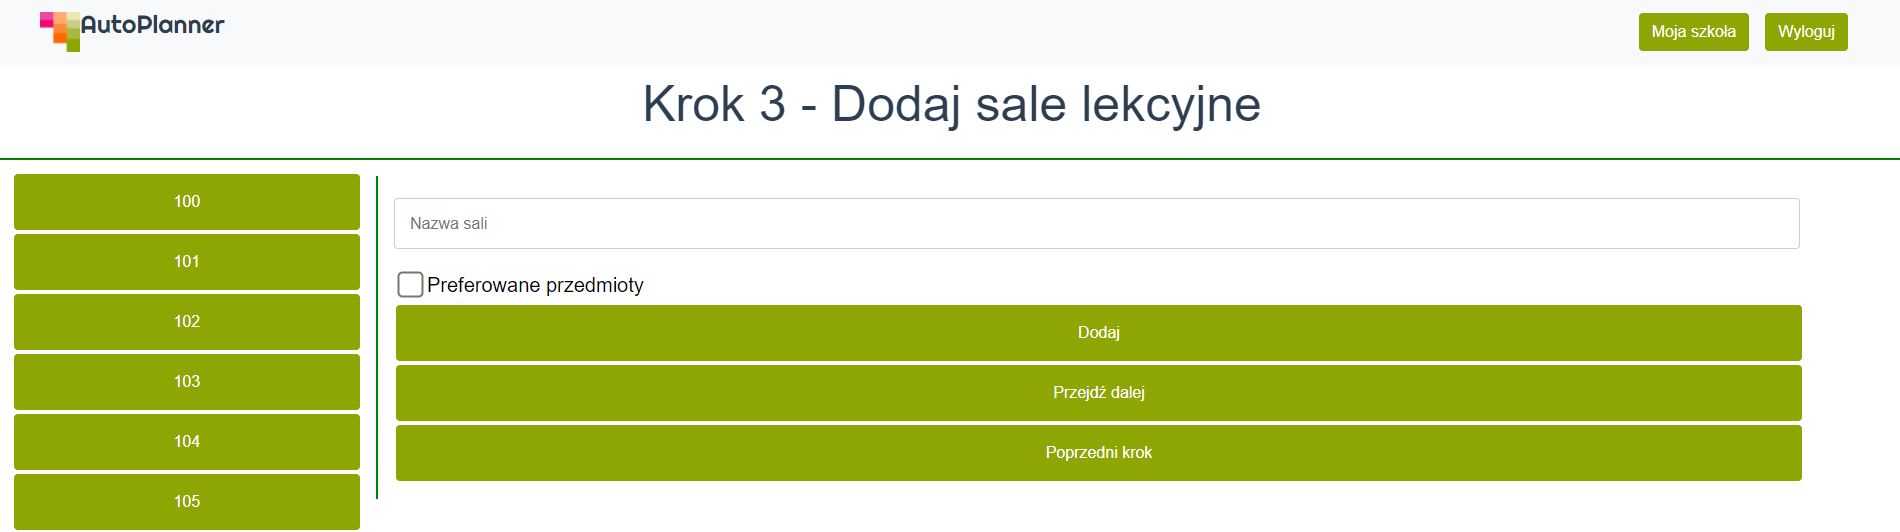
\includegraphics[width=\textwidth]{figures/classroom}
\caption{Aplikacja internetowa -- Widok dodawania sali lekcyjnych}\label{rys:classroom}
\end{figure}
\section{Dodawanie klas}
Ostatnim etapem w procesie dodawania niezbędnych danych jest wprowadzenie parametrów klas~(zob.~rysunek~\ref{rys:class}). Każda klasa musi posiadać nazwę oraz listę przedmiotów, które mają się pojawić w jej planie zajęć. Każdy element listy musi zawierać nazwę przedmiotu, liczbę godzin lekcyjnych w tygodniu przeznaczonych na przedmiot oraz opcjonalnie prowadzącego przedmiot. Brak wyboru nauczyciela umożliwia przypisanie zajęć dowolnemu prowadzącemu dany przedmiot.
\begin{figure}[!ht]
\centering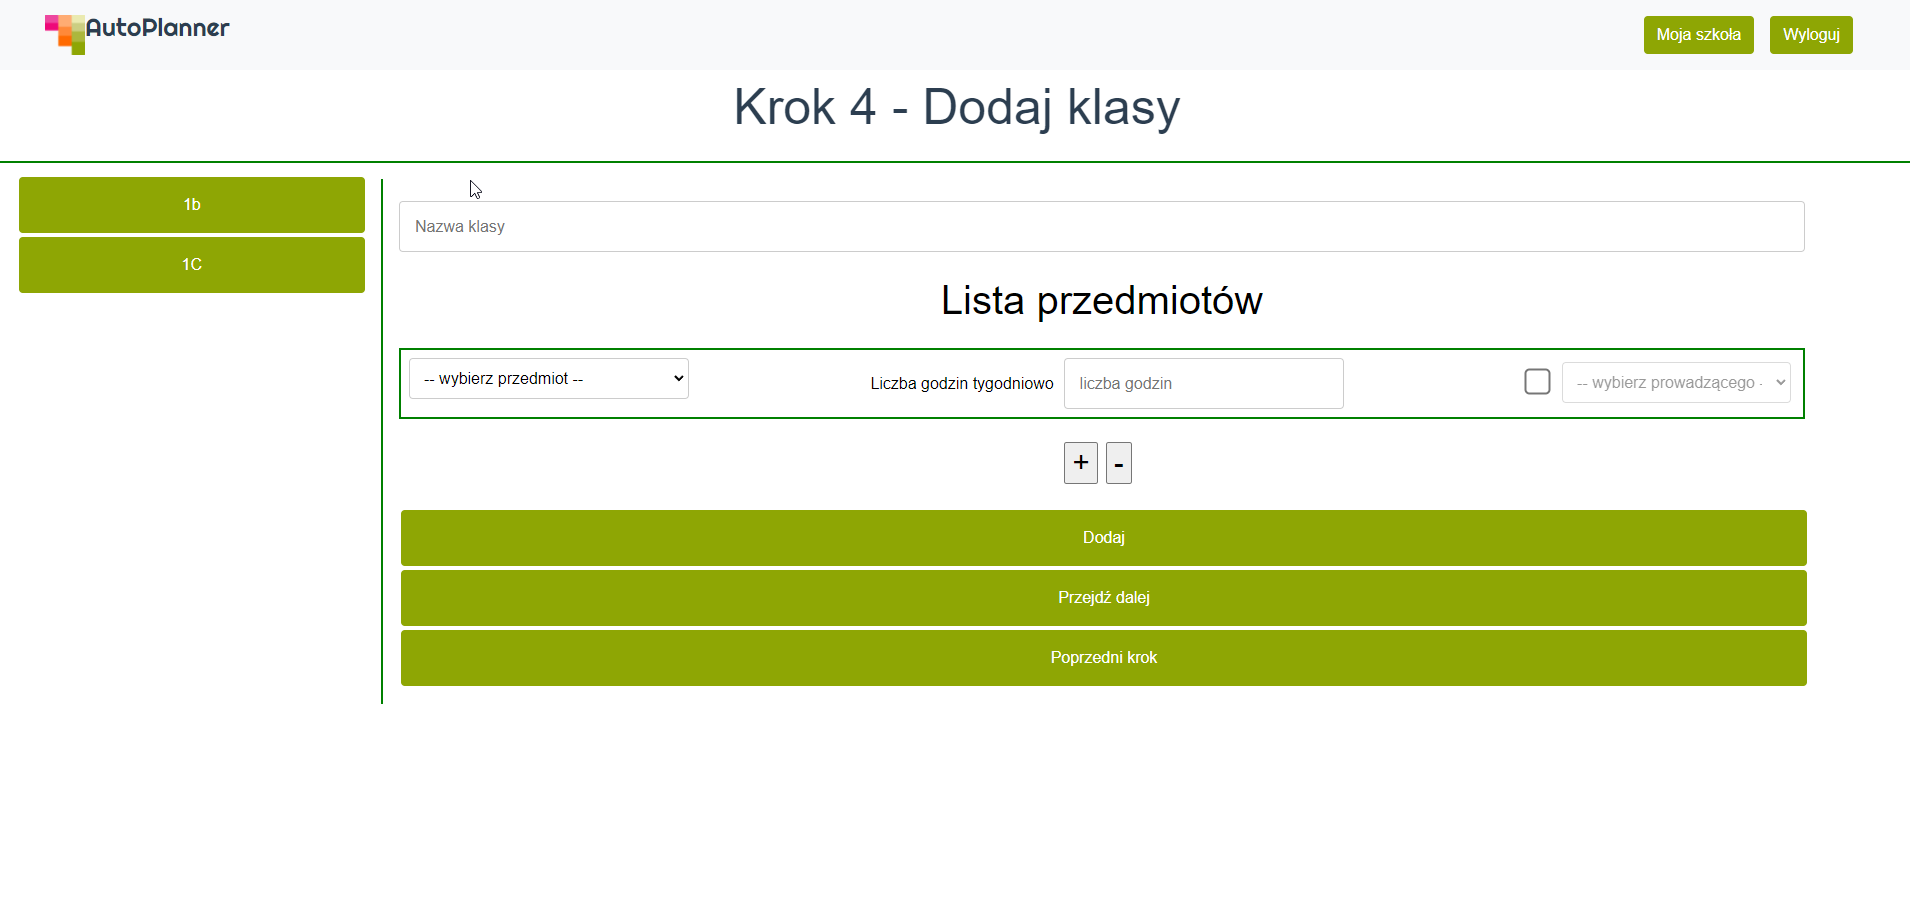
\includegraphics[width=\textwidth]{figures/class}
\caption{Aplikacja internetowa -- Widok dodawania klas}\label{rys:class}
\end{figure}
\section{Edycja danych}
Dla czterech powyższych ekranów istnieją odpowiadające im ekrany edycji danych. Ze względu na ich analogiczną budowę ich struktura zostanie omówiona na bazie widoku edycji danych nauczyciela~(zob.~rysunek~\ref{rys:edit}). Przejście do tego ekranu umożliwiają przyciski znajdujące się po prawej stronie widoku dodawania nauczycieli. Przyciski te są wciąż obecne w widoku edycji i pozwalają na przechodzenie pomiędzy danymi poszczególnych osób bez zapisywania wprowadzonych zmian.

\begin{figure}[h]
\centering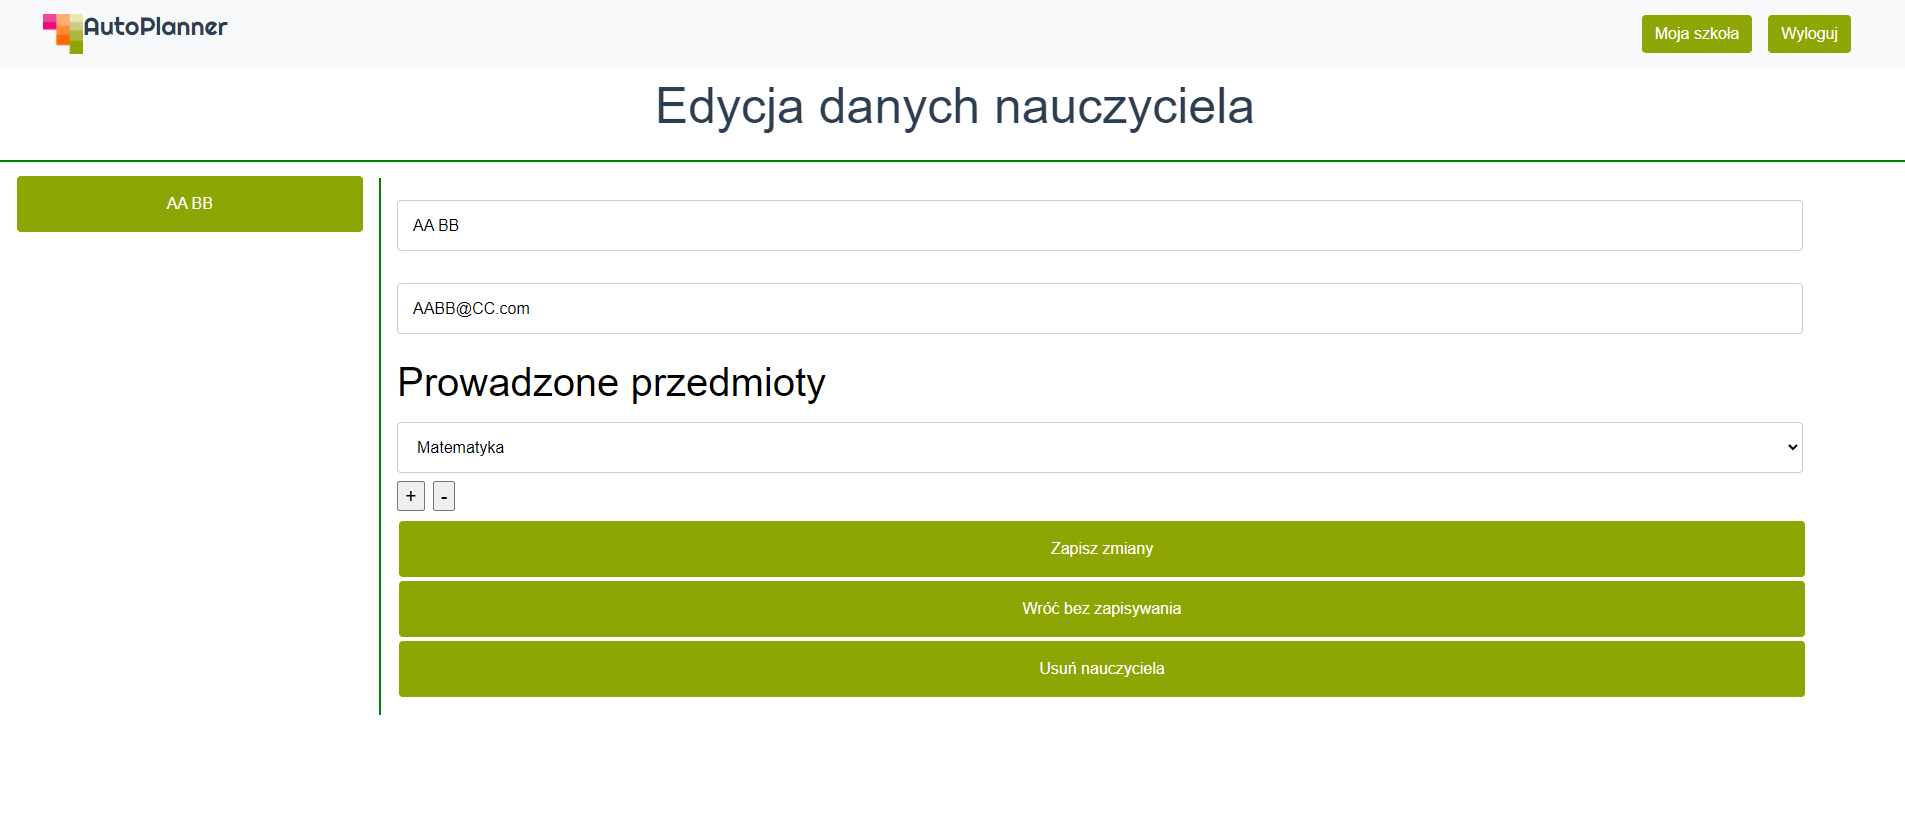
\includegraphics[width=\textwidth]{figures/edit}
\caption{Aplikacja internetowa -- Widok edycji danych nauczyciela}\label{rys:edit}
\end{figure}

 W chwili przejścia do ekranu edycji pola z danymi zostają uzupełnione pierwotnie wprowadzonymi informacjami o nauczycielu. Takie rozwiązanie ma celu zapobieganie konieczności ponownego wprowadzania wszystkich danych, w przypadku gdy tylko niektóre z nich wymagają zmian. Przyciski u dołu pozwalają na zapisanie wprowadzonych zmian, powrót do ekranu dodawania nauczycieli lub całkowite usunięcie nauczyciela z bazy danych.
